\question (中南大学,2003年)某二叉树结点的中序序列为BDAECF,后序序列为DBEFCA,则该二叉树对应的森林包括(
)棵树
\par\twoch{1}{2}{\textcolor{red}{3}}{4}
\begin{solution}先还原二叉树,从后序序列可知根为A,那么左子树的中序就为BD,右子树的中序为ECF,左子树的后序为DB,右子树的后序为EFC;可再得,左子树的根为B,D为右孩子;右子树的根为C,左孩子为E,右孩子为F。画出示意图,如下图所示。
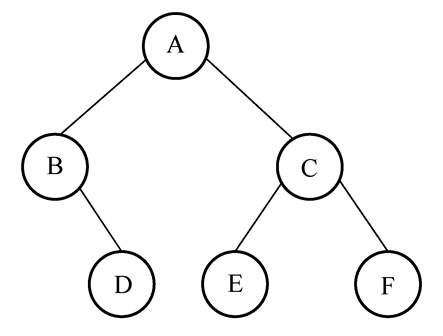
\includegraphics[width=2.08333in,height=2.08333in]{computerassets/bd459a854ebd7c5ece063bf107b6f012.jpeg}
可以直接看根结点有几个兄弟,兄弟数+1(因为还有根结点本身)即为树的个数。
下面给出转换为森林后的示意图:
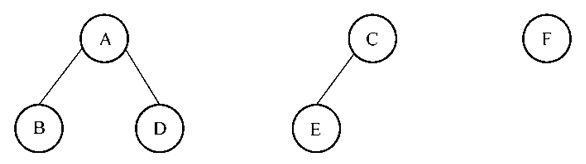
\includegraphics[width=2.08333in,height=2.08333in]{computerassets/02d7f3ef22c9ad637a111d6ad3d5cc3d.jpeg}
综上,本题选C。
\end{solution}
\question (哈尔滨工程大学,2004年)树用孩子兄弟表示法,每个结点有两个指针域,分别指向``第一个孩子''和``下一个兄弟''。若指向``下一个兄弟''的指针有n个为空,则该树有(
)个非终端结点
\par\twoch{[n/2]}{\textcolor{red}{n-1}}{n}{n+1}
\begin{solution}举特例,只有一个根结点的情况下,``下一个兄弟''的指针有1个为空,有0个非终端结点,可排除A、C和D。
下面来求证一下,在特例基础上,增加一个``第一个孩子'',则空的``下一个兄弟''的指针加1,非终端结点加1;而增加一个``下一个兄弟'',则空的``下一个兄弟''的指针数不变,非终端结点数不变,即非终端结点数和空的``下一个兄弟''指针相关,为n-1。
\end{solution}
\question (南京林业大学,2005年)设森林F对应的二叉树为B,B有m个结点,B的根为p,p的右子树结点个数为n,森林F的第一棵树的结点个数是(
)
\par\twoch{\textcolor{red}{m-n}}{m-n+1}{n+1}{条件不足,无法确定}
\begin{solution}第一棵树的结点转换为二叉树后,都在B的左子树之中,而p的右子树个数为n,那么只需要计算左子树的个数即可,即为m-n。
\end{solution}
\question 将森林转换为对应的二叉树,若在二叉树中,结点u是结点v的父结点的父结点,则在原来的森林中,u和v可能具有的关系是(
~)。 \ding{192}.父子关系 ~ \ding{193}.兄弟关系 \ding{194}.u的父结点与v的父结点是兄弟关系
\par\twoch{只有\ding{193}}{\textcolor{red}{\ding{192}和\ding{193}}}{\ding{192}和\ding{194}}{\ding{192}、\ding{193}和\ding{194}}
\begin{solution}若u和v的关系如下图a所示,在二叉树中,结点u是结点v的父结点的父结点,则根据左孩子右兄弟原则,在森林中:u和v是父子关系。
若u和v的关系如下图b所示,在二叉树中,结点u是v的父结点的父结点,则根据左孩子右兄弟原则,在森林中:u和v是兄弟关系。
若u和v的关系如下图c所示,在森林中:u的父结点与v的父结点是兄弟关系,转换成二叉树后,y为x的右孩子,u不可能是v的父结点的父结点。
【总结】 做这类比较抽象的题目时,举例子是最直观的解法。
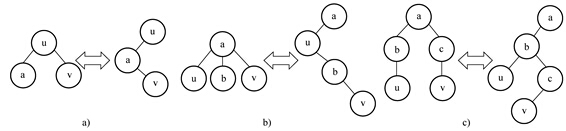
\includegraphics[width=3.43750in,height=0.79167in]{computerassets/c988dc89d58b0e157aa15f8cdbc93ba0.jpeg}
\end{solution}
\question 将森林F转化为对应的二叉树T,F中叶结点的个数等于( )
\par\twoch{T中叶结点的个数}{T中度为1的结点个数}{\textcolor{red}{T中左孩子指针为空的结点个数}}{T中右孩子指针为空的结点个数}
\begin{solution}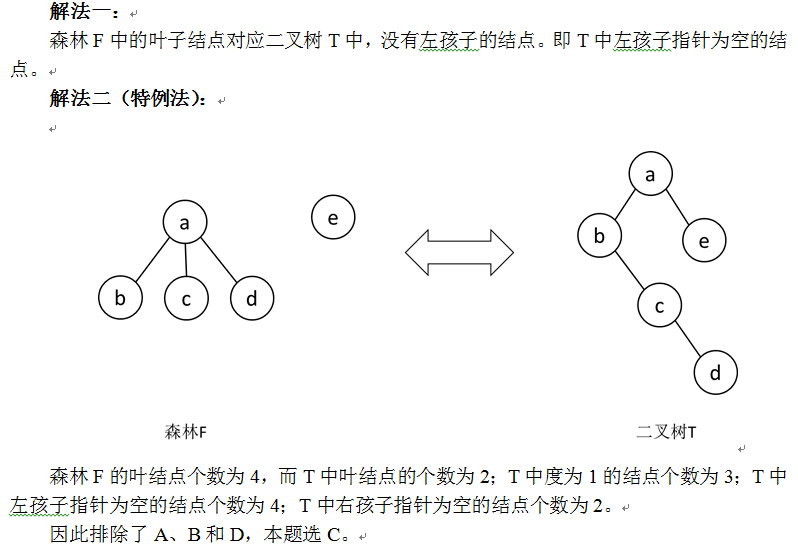
\includegraphics[width=8.31250in,height=5.72917in]{computerassets/8e82dd8ce320967b382ec04f01be2a5d.jpeg}
\end{solution}
\question (江苏大学,2005年)设森林F中有3棵树,第一、第二、第三棵树的节点个数分别为9、8、7。与森林F对应的二叉树根节点的右子树上的结点个数是(
)
\par\twoch{16}{\textcolor{red}{15}}{7}{17}
\begin{solution}右子树为第二、三棵树的节点个数之和
\end{solution}
\question (南京邮电大学,2005年)设X是树T中的一个非根节点,B是T所对应的二叉树。在B中,X是其双亲的右孩子,下列结论正确的是(
)
\par\fourch{在树T中,X是其双亲的第一个孩子}{在树T中,X一定无右边兄弟}{在树T中,X一定是叶子节点}{\textcolor{red}{在树T中,X一定有左边兄弟}}
\begin{solution}树转化为二叉树过程中,若X是非根节点,二叉树的右孩子对应原树节点的右兄弟。故X一定有左边兄弟
\end{solution}
